%File: formatting-instructions-latex-2026.tex
%release 2026.0
\documentclass[letterpaper]{article} % DO NOT CHANGE THIS
\usepackage{aaai2026}  % DO NOT CHANGE THIS
\usepackage{times}  % DO NOT CHANGE THIS
\usepackage{helvet}  % DO NOT CHANGE THIS
\usepackage{courier}  % DO NOT CHANGE THIS
\usepackage[hyphens]{url}  % DO NOT CHANGE THIS
\usepackage{graphicx} % DO NOT CHANGE THIS
\urlstyle{rm} % DO NOT CHANGE THIS
\def\UrlFont{\rm}  % DO NOT CHANGE THIS
\usepackage{natbib}  % DO NOT CHANGE THIS AND DO NOT ADD ANY OPTIONS TO IT
\usepackage{caption} % DO NOT CHANGE THIS AND DO NOT ADD ANY OPTIONS TO IT
\frenchspacing  % DO NOT CHANGE THIS
\setlength{\pdfpagewidth}{8.5in}  % DO NOT CHANGE THIS
\setlength{\pdfpageheight}{11in}  % DO NOT CHANGE THIS
%
% These are recommended to typeset algorithms but not required. See the subsubsection on algorithms. Remove them if you don't have algorithms in your paper.
\usepackage{algorithm}
\usepackage{algorithmic}

%
% These are are recommended to typeset listings but not required. See the subsubsection on listing. Remove this block if you don't have listings in your paper.
\usepackage{newfloat}
\usepackage{listings}
\DeclareCaptionStyle{ruled}{labelfont=normalfont,labelsep=colon,strut=off} % DO NOT CHANGE THIS
\lstset{%
	basicstyle={\footnotesize\ttfamily},% footnotesize acceptable for monospace
	numbers=left,numberstyle=\footnotesize,xleftmargin=2em,% show line numbers, remove this entire line if you don't want the numbers.
	aboveskip=0pt,belowskip=0pt,%
	showstringspaces=false,tabsize=2,breaklines=true}
\floatstyle{ruled}
\newfloat{listing}{tb}{lst}{}
\floatname{listing}{Listing}
%
% Keep the \pdfinfo as shown here. There's no need
% for you to add the /Title and /Author tags.
\pdfinfo{
/TemplateVersion (2026.1)
}

% DISALLOWED PACKAGES
% \usepackage{authblk} -- This package is specifically forbidden
% \usepackage{balance} -- This package is specifically forbidden
% \usepackage{color (if used in text)
% \usepackage{CJK} -- This package is specifically forbidden
% \usepackage{float} -- This package is specifically forbidden
% \usepackage{flushend} -- This package is specifically forbidden
% \usepackage{fontenc} -- This package is specifically forbidden
% \usepackage{fullpage} -- This package is specifically forbidden
% \usepackage{geometry} -- This package is specifically forbidden
% \usepackage{grffile} -- This package is specifically forbidden
% \usepackage{hyperref} -- This package is specifically forbidden
% \usepackage{navigator} -- This package is specifically forbidden
% (or any other package that embeds links such as navigator or hyperref)
% \indentfirst} -- This package is specifically forbidden
% \layout} -- This package is specifically forbidden
% \multicol} -- This package is specifically forbidden
% \nameref} -- This package is specifically forbidden
% \usepackage{savetrees} -- This package is specifically forbidden
% \usepackage{setspace} -- This package is specifically forbidden
% \usepackage{stfloats} -- This package is specifically forbidden
% \usepackage{tabu} -- This package is specifically forbidden
% \usepackage{titlesec} -- This package is specifically forbidden
% \usepackage{tocbibind} -- This package is specifically forbidden
% \usepackage{ulem} -- This package is specifically forbidden
% \usepackage{wrapfig} -- This package is specifically forbidden
% DISALLOWED COMMANDS
% \nocopyright -- Your paper will not be published if you use this command
% \addtolength -- This command may not be used
% \balance -- This command may not be used
% \baselinestretch -- Your paper will not be published if you use this command
% \clearpage -- No page breaks of any kind may be used for the final version of your paper
% \columnsep -- This command may not be used
% \newpage -- No page breaks of any kind may be used for the final version of your paper
% \pagebreak -- No page breaks of any kind may be used for the final version of your paperr
% \pagestyle -- This command may not be used
% \tiny -- This is not an acceptable font size.
% \vspace{- -- No negative value may be used in proximity of a caption, figure, table, section, subsection, subsubsection, or reference
% \vskip{- -- No negative value may be used to alter spacing above or below a caption, figure, table, section, subsection, subsubsection, or reference

\setcounter{secnumdepth}{0} %May be changed to 1 or 2 if section numbers are desired.

% The file aaai2026.sty is the style file for AAAI Press
% proceedings, working notes, and technical reports.
%

% Title

% Your title must be in mixed case, not sentence case.
% That means all verbs (including short verbs like be, is, using,and go),
% nouns, adverbs, adjectives should be capitalized, including both words in hyphenated terms, while
% articles, conjunctions, and prepositions are lower case unless they
% directly follow a colon or long dash
\title{AAAI Press Formatting Instructions \\for Authors Using \LaTeX{} --- A Guide}
\author{
    %Authors
    % All authors must be in the same font size and format.
    Written by AAAI Press Staff\textsuperscript{\rm 1}\thanks{With help from the AAAI Publications Committee.}\\
    AAAI Style Contributions by Pater Patel Schneider,
    Sunil Issar,\\
    J. Scott Penberthy,
    George Ferguson,
    Hans Guesgen,
    Francisco Cruz\equalcontrib,
    Marc Pujol-Gonzalez\equalcontrib
}
\affiliations{
    %Afiliations
    \textsuperscript{\rm 1}Association for the Advancement of Artificial Intelligence\\
    % If you have multiple authors and multiple affiliations
    % use superscripts in text and roman font to identify them.
    % For example,

    % Sunil Issar\textsuperscript{\rm 2}, 
    % J. Scott Penberthy\textsuperscript{\rm 3}, 
    % George Ferguson\textsuperscript{\rm 4},
    % Hans Guesgen\textsuperscript{\rm 5}
    % Note that the comma should be placed after the superscript

    1101 Pennsylvania Ave, NW Suite 300\\
    Washington, DC 20004 USA\\
    % email address must be in roman text type, not monospace or sans serif
    proceedings-questions@aaai.org
%
% See more examples next
}

%Example, Single Author, ->> remove \iffalse,\fi and place them surrounding AAAI title to use it
\iffalse
\title{My Publication Title --- Single Author}
\author {
    Author Name
}
\affiliations{
    Affiliation\\
    Affiliation Line 2\\
    name@example.com
}
\fi

\iffalse
%Example, Multiple Authors, ->> remove \iffalse,\fi and place them surrounding AAAI title to use it
\title{My Publication Title --- Multiple Authors}
\author {
    % Authors
    First Author Name\textsuperscript{\rm 1,\rm 2},
    Second Author Name\textsuperscript{\rm 2},
    Third Author Name\textsuperscript{\rm 1}
}
\affiliations {
    % Affiliations
    \textsuperscript{\rm 1}Affiliation 1\\
    \textsuperscript{\rm 2}Affiliation 2\\
    firstAuthor@affiliation1.com, secondAuthor@affilation2.com, thirdAuthor@affiliation1.com
}
\fi


% REMOVE THIS: bibentry
% This is only needed to show inline citations in the guidelines document. You should not need it and can safely delete it.
\usepackage{bibentry}
% END REMOVE bibentry

\begin{document}

\maketitle

\begin{abstract}
AAAI creates proceedings, working notes, and technical reports directly from electronic source furnished by the authors. To ensure that all papers in the publication have a uniform appearance, authors must adhere to the following instructions.
\end{abstract}

% Uncomment the following to link to your code, datasets, an extended version or similar.
% You must keep this block between (not within) the abstract and the main body of the paper.
\begin{links}
    \link{Code}{https://aaai.org/example/code}
    \link{Datasets}{https://aaai.org/example/datasets}
    \link{Extended version}{https://aaai.org/example/extended-version}
\end{links}

\section{Introduction}

Congratulations on having a paper selected for inclusion in an AAAI Press proceedings or technical report! This document details the requirements necessary to get your accepted paper published using PDF\LaTeX{}. If you are using Microsoft Word, instructions are provided in a different document. AAAI Press does not support any other formatting software.

The instructions herein are provided as a general guide for experienced \LaTeX{} users. If you do not know how to use \LaTeX{}, please obtain assistance locally. AAAI cannot provide you with support and the accompanying style files are \textbf{not} guaranteed to work. If the results you obtain are not in accordance with the specifications you received, you must correct your source file to achieve the correct result.

These instructions are generic. Consequently, they do not include specific dates, page charges, and so forth. Please consult your specific written conference instructions for details regarding your submission. Please review the entire document for specific instructions that might apply to your particular situation. All authors must comply with the following:

\begin{itemize}
\item You must use the 2026 AAAI Press \LaTeX{} style file and the aaai2026.bst bibliography style files, which are located in the 2026 AAAI Author Kit (aaai2026.sty, aaai2026.bst).
\item You must complete, sign, and return by the deadline the AAAI copyright form (unless directed by AAAI Press to use the AAAI Distribution License instead).
\item You must read and format your paper source and PDF according to the formatting instructions for authors.
\item You must submit your electronic files and abstract using our electronic submission form \textbf{on time.}
\item You must pay any required page or formatting charges to AAAI Press so that they are received by the deadline.
\item You must check your paper before submitting it, ensuring that it compiles without error, and complies with the guidelines found in the AAAI Author Kit.
\end{itemize}

\section{Copyright}
All papers submitted for publication by AAAI Press must be accompanied by a valid signed copyright form. They must also contain the AAAI copyright notice at the bottom of the first page of the paper. There are no exceptions to these requirements. If you fail to provide us with a signed copyright form or disable the copyright notice, we will be unable to publish your paper. There are \textbf{no exceptions} to this policy. You will find a PDF version of the AAAI copyright form in the AAAI AuthorKit. Please see the specific instructions for your conference for submission details.

\section{Formatting Requirements in Brief}
We need source and PDF files that can be used in a variety of ways and can be output on a variety of devices. The design and appearance of the paper is strictly governed by the aaai style file (aaai2026.sty).
\textbf{You must not make any changes to the aaai style file, nor use any commands, packages, style files, or macros within your own paper that alter that design, including, but not limited to spacing, floats, margins, fonts, font size, and appearance.} AAAI imposes requirements on your source and PDF files that must be followed. Most of these requirements are based on our efforts to standardize conference manuscript properties and layout. All papers submitted to AAAI for publication will be recompiled for standardization purposes. Consequently, every paper submission must comply with the following requirements:

\begin{itemize}
\item Your .tex file must compile in PDF\LaTeX{} --- (you may not include .ps or .eps figure files.)
\item All fonts must be embedded in the PDF file --- including your figures.
\item Modifications to the style file, whether directly or via commands in your document may not ever be made, most especially when made in an effort to avoid extra page charges or make your paper fit in a specific number of pages.
\item No type 3 fonts may be used (even in illustrations).
\item You may not alter the spacing above and below captions, figures, headings, and subheadings.
\item You may not alter the font sizes of text elements, footnotes, heading elements, captions, or title information (for references and mathematics, please see the limited exceptions provided herein).
\item You may not alter the line spacing of text.
\item Your title must follow Title Case capitalization rules (not sentence case).
\item \LaTeX{} documents must use the Times or Nimbus font package (you may not use Computer Modern for the text of your paper).
\item No \LaTeX{} 209 documents may be used or submitted.
\item Your source must not require use of fonts for non-Roman alphabets within the text itself. If your paper includes symbols in other languages (such as, but not limited to, Arabic, Chinese, Hebrew, Japanese, Thai, Russian and other Cyrillic languages), you must restrict their use to bit-mapped figures. Fonts that require non-English language support (CID and Identity-H) must be converted to outlines or 300 dpi bitmap or removed from the document (even if they are in a graphics file embedded in the document).
\item Two-column format in AAAI style is required for all papers.
\item The paper size for final submission must be US letter without exception.
\item The source file must exactly match the PDF.
\item The document margins may not be exceeded (no overfull boxes).
\item The number of pages and the file size must be as specified for your event.
\item No document may be password protected.
\item Neither the PDFs nor the source may contain any embedded links or bookmarks (no hyperref or navigator packages).
\item Your source and PDF must not have any page numbers, footers, or headers (no pagestyle commands).
\item Your PDF must be compatible with Acrobat 5 or higher.
\item Your \LaTeX{} source file (excluding references) must consist of a \textbf{single} file (use of the ``input" command is not allowed.
\item Your graphics must be sized appropriately outside of \LaTeX{} (do not use the ``clip" or ``trim'' command) .
\end{itemize}

If you do not follow these requirements, your paper will be returned to you to correct the deficiencies.

\section{What Files to Submit}
You must submit the following items to ensure that your paper is published:
\begin{itemize}
\item A fully-compliant PDF file.
\item Your \LaTeX{} source file submitted as a \textbf{single} .tex file (do not use the ``input" command to include sections of your paper --- every section must be in the single source file). (The only allowable exception is .bib file, which should be included separately).
\item The bibliography (.bib) file(s).
\item Your source must compile on our system, which includes only standard \LaTeX{} 2020 TeXLive support files.
\item Only the graphics files used in compiling paper.
\item The \LaTeX{}-generated files (e.g. .aux,  .bbl file, PDF, etc.).
\end{itemize}

Your \LaTeX{} source will be reviewed and recompiled on our system (if it does not compile, your paper will be returned to you. \textbf{Do not submit your source in multiple text files.} Your single \LaTeX{} source file must include all your text, your bibliography (formatted using aaai2026.bst), and any custom macros.

Your files should work without any supporting files (other than the program itself) on any computer with a standard \LaTeX{} distribution.

\textbf{Do not send files that are not actually used in the paper.} Avoid including any files not needed for compiling your paper, including, for example, this instructions file, unused graphics files, style files, additional material sent for the purpose of the paper review, intermediate build files and so forth.
\textbf{Obsolete style files.} The commands for some common packages (such as some used for algorithms), may have changed. Please be certain that you are not compiling your paper using old or obsolete style files.

\textbf{Final Archive.} Place your source files in a single archive which should be compressed using .zip. The final file size may not exceed 10 MB.
Name your source file with the last (family) name of the first author, even if that is not you.


\section{Using \LaTeX{} to Format Your Paper}

The latest version of the AAAI style file is available on AAAI's website. Download this file and place it in the \TeX\ search path. Placing it in the same directory as the paper should also work. You must download the latest version of the complete AAAI Author Kit so that you will have the latest instruction set and style file.

\subsection{Document Preamble}

In the \LaTeX{} source for your paper, you \textbf{must} place the following lines as shown in the example in this subsection. This command set-up is for three authors. Add or subtract author and address lines as necessary, and uncomment the portions that apply to you. In most instances, this is all you need to do to format your paper in the Times font. The helvet package will cause Helvetica to be used for sans serif. These files are part of the PSNFSS2e package, which is freely available from many Internet sites (and is often part of a standard installation).

Leave the setcounter for section number depth commented out and set at 0 unless you want to add section numbers to your paper. If you do add section numbers, you must uncomment this line and change the number to 1 (for section numbers), or 2 (for section and subsection numbers). The style file will not work properly with numbering of subsubsections, so do not use a number higher than 2.

\subsubsection{The Following Must Appear in Your Preamble}
\begin{quote}
\begin{scriptsize}\begin{verbatim}
\documentclass[letterpaper]{article}
% DO NOT CHANGE THIS
\usepackage{aaai2026} % DO NOT CHANGE THIS
\usepackage{times} % DO NOT CHANGE THIS
\usepackage{helvet} % DO NOT CHANGE THIS
\usepackage{courier} % DO NOT CHANGE THIS
\usepackage[hyphens]{url} % DO NOT CHANGE THIS
\usepackage{graphicx} % DO NOT CHANGE THIS
\urlstyle{rm} % DO NOT CHANGE THIS
\def\UrlFont{\rm} % DO NOT CHANGE THIS
\usepackage{graphicx}  % DO NOT CHANGE THIS
\usepackage{natbib}  % DO NOT CHANGE THIS
\usepackage{caption}  % DO NOT CHANGE THIS
\frenchspacing % DO NOT CHANGE THIS
\setlength{\pdfpagewidth}{8.5in} % DO NOT CHANGE THIS
\setlength{\pdfpageheight}{11in} % DO NOT CHANGE THIS
%
% Keep the \pdfinfo as shown here. There's no need
% for you to add the /Title and /Author tags.
\pdfinfo{
/TemplateVersion (2026.1)
}
\end{verbatim}\end{scriptsize}
\end{quote}

\subsection{Preparing Your Paper}

After the preamble above, you should prepare your paper as follows:
\begin{quote}
\begin{scriptsize}\begin{verbatim}
\begin{document}
\maketitle
\begin{abstract}
%...
\end{abstract}\end{verbatim}\end{scriptsize}
\end{quote}

\noindent If you want to add links to the paper's code, dataset(s), and extended version or similar this is the place to add them, within a \emph{links} environment:
\begin{quote}%
\begin{scriptsize}\begin{verbatim}
\begin{links}
  \link{Code}{https://aaai.org/example/guidelines}
  \link{Datasets}{https://aaai.org/example/datasets}
  \link{Extended version}{https://aaai.org/example}
\end{links}\end{verbatim}\end{scriptsize}
\end{quote}

\noindent You should then continue with the body of your paper. Your paper must conclude with the references, which should be inserted as follows:
\begin{quote}
\begin{scriptsize}\begin{verbatim}
% References and End of Paper
% These lines must be placed at the end of your paper
\bibliography{Bibliography-File}
\end{document}
\end{verbatim}\end{scriptsize}
\end{quote}


\begin{quote}
\begin{scriptsize}\begin{verbatim}
\begin{document}\\
\maketitle\\
...\\
\bibliography{Bibliography-File}\\
\end{document}\\
\end{verbatim}\end{scriptsize}
\end{quote}

\subsection{Commands and Packages That May Not Be Used}
\begin{table*}[t]
\centering

\begin{tabular}{l|l|l|l}
\textbackslash abovecaption &
\textbackslash abovedisplay &
\textbackslash addevensidemargin &
\textbackslash addsidemargin \\
\textbackslash addtolength &
\textbackslash baselinestretch &
\textbackslash belowcaption &
\textbackslash belowdisplay \\
\textbackslash break &
\textbackslash clearpage &
\textbackslash clip &
\textbackslash columnsep \\
\textbackslash float &
\textbackslash input &
\textbackslash input &
\textbackslash linespread \\
\textbackslash newpage &
\textbackslash pagebreak &
\textbackslash renewcommand &
\textbackslash setlength \\
\textbackslash text height &
\textbackslash tiny &
\textbackslash top margin &
\textbackslash trim \\
\textbackslash vskip\{- &
\textbackslash vspace\{- \\
\end{tabular}
%}
\caption{Commands that must not be used}
\label{table1}
\end{table*}

\begin{table}[t]
\centering
%\resizebox{.95\columnwidth}{!}{
\begin{tabular}{l|l|l|l}
    authblk & babel & cjk & dvips \\
    epsf & epsfig & euler & float \\
    fullpage & geometry & graphics & hyperref \\
    layout & linespread & lmodern & maltepaper \\
    navigator & pdfcomment & pgfplots & psfig \\
    pstricks & t1enc & titlesec & tocbind \\
    ulem
\end{tabular}
\caption{LaTeX style packages that must not be used.}
\label{table2}
\end{table}

There are a number of packages, commands, scripts, and macros that are incompatable with aaai2026.sty. The common ones are listed in tables \ref{table1} and \ref{table2}. Generally, if a command, package, script, or macro alters floats, margins, fonts, sizing, linespacing, or the presentation of the references and citations, it is unacceptable. Note that negative vskip and vspace may not be used except in certain rare occurances, and may never be used around tables, figures, captions, sections, subsections, subsubsections, or references.


\subsection{Page Breaks}
For your final camera ready copy, you must not use any page break commands. References must flow directly after the text without breaks. Note that some conferences require references to be on a separate page during the review process. AAAI Press, however, does not require this condition for the final paper.


\subsection{Paper Size, Margins, and Column Width}
Papers must be formatted to print in two-column format on 8.5 x 11 inch US letter-sized paper. The margins must be exactly as follows:
\begin{itemize}
\item Top margin: .75 inches
\item Left margin: .75 inches
\item Right margin: .75 inches
\item Bottom margin: 1.25 inches
\end{itemize}


The default paper size in most installations of \LaTeX{} is A4. However, because we require that your electronic paper be formatted in US letter size, the preamble we have provided includes commands that alter the default to US letter size. Please note that using any other package to alter page size (such as, but not limited to the Geometry package) will result in your final paper being returned to you for correction.


\subsubsection{Column Width and Margins.}
To ensure maximum readability, your paper must include two columns. Each column should be 3.3 inches wide (slightly more than 3.25 inches), with a .375 inch (.952 cm) gutter of white space between the two columns. The aaai2026.sty file will automatically create these columns for you.

\subsection{Overlength Papers}
If your paper is too long and you resort to formatting tricks to make it fit, it is quite likely that it will be returned to you. The best way to retain readability if the paper is overlength is to cut text, figures, or tables. There are a few acceptable ways to reduce paper size that don't affect readability. First, turn on \textbackslash frenchspacing, which will reduce the space after periods. Next, move all your figures and tables to the top of the page. Consider removing less important portions of a figure. If you use \textbackslash centering instead of \textbackslash begin\{center\} in your figure environment, you can also buy some space. For mathematical environments, you may reduce fontsize {\bf but not below 6.5 point}.


Commands that alter page layout are forbidden. These include \textbackslash columnsep,  \textbackslash float, \textbackslash topmargin, \textbackslash topskip, \textbackslash textheight, \textbackslash textwidth, \textbackslash oddsidemargin, and \textbackslash evensizemargin (this list is not exhaustive). If you alter page layout, you will be required to pay the page fee. Other commands that are questionable and may cause your paper to be rejected include \textbackslash parindent, and \textbackslash parskip. Commands that alter the space between sections are forbidden. The title sec package is not allowed. Regardless of the above, if your paper is obviously ``squeezed" it is not going to to be accepted. Options for reducing the length of a paper include reducing the size of your graphics, cutting text, or paying the extra page charge (if it is offered).


\subsection{Type Font and Size}
Your paper must be formatted in Times Roman or Nimbus. We will not accept papers formatted using Computer Modern or Palatino or some other font as the text or heading typeface. Sans serif, when used, should be Courier. Use Symbol or Lucida or Computer Modern for \textit{mathematics only. }

Do not use type 3 fonts for any portion of your paper, including graphics. Type 3 bitmapped fonts are designed for fixed resolution printers. Most print at 300 dpi even if the printer resolution is 1200 dpi or higher. They also often cause high resolution imagesetter devices to crash. Consequently, AAAI will not accept electronic files containing obsolete type 3 fonts. Files containing those fonts (even in graphics) will be rejected. (Authors using blackboard symbols must avoid packages that use type 3 fonts.)

Fortunately, there are effective workarounds that will prevent your file from embedding type 3 bitmapped fonts. The easiest workaround is to use the required times, helvet, and courier packages with \LaTeX{}2e. (Note that papers formatted in this way will still use Computer Modern for the mathematics. To make the math look good, you'll either have to use Symbol or Lucida, or you will need to install type 1 Computer Modern fonts --- for more on these fonts, see the section ``Obtaining Type 1 Computer Modern.")

If you are unsure if your paper contains type 3 fonts, view the PDF in Acrobat Reader. The Properties/Fonts window will display the font name, font type, and encoding properties of all the fonts in the document. If you are unsure if your graphics contain type 3 fonts (and they are PostScript or encapsulated PostScript documents), create PDF versions of them, and consult the properties window in Acrobat Reader.

The default size for your type must be ten-point with twelve-point leading (line spacing). Start all pages (except the first) directly under the top margin. (See the next section for instructions on formatting the title page.) Indent ten points when beginning a new paragraph, unless the paragraph begins directly below a heading or subheading.


\subsubsection{Obtaining Type 1 Computer Modern for \LaTeX{}.}

If you use Computer Modern for the mathematics in your paper (you cannot use it for the text) you may need to download type 1 Computer fonts. They are available without charge from the American Mathematical Society:
http://www.ams.org/tex/type1-fonts.html.

\subsubsection{Nonroman Fonts.}
If your paper includes symbols in other languages (such as, but not limited to, Arabic, Chinese, Hebrew, Japanese, Thai, Russian and other Cyrillic languages), you must restrict their use to bit-mapped figures.

\subsection{Title and Authors}
Your title must appear centered over both text columns in sixteen-point bold type (twenty-four point leading). The title must be written in Title Case according to the Chicago Manual of Style rules. The rules are a bit involved, but in general verbs (including short verbs like be, is, using, and go), nouns, adverbs, adjectives, and pronouns should be capitalized, (including both words in hyphenated terms), while articles, conjunctions, and prepositions are lower case unless they directly follow a colon or long dash. You can use the online tool \url{https://titlecaseconverter.com/} to double-check the proper capitalization (select the "Chicago" style and mark the "Show explanations" checkbox).

Author's names should appear below the title of the paper, centered in twelve-point type (with fifteen point leading), along with affiliation(s) and complete address(es) (including electronic mail address if available) in nine-point roman type (the twelve point leading). You should begin the two-column format when you come to the abstract.

\subsubsection{Formatting Author Information.}
Author information has to be set according to the following specification depending if you have one or more than one affiliation. You may not use a table nor may you employ the \textbackslash authorblk.sty package. For one or several authors from the same institution, please separate them with commas and write all affiliation directly below (one affiliation per line) using the macros \textbackslash author and \textbackslash affiliations:

\begin{quote}\begin{scriptsize}\begin{verbatim}
\author{
    Author 1, ..., Author n\\
}
\affiliations {
    Address line\\
    ... \\
    Address line\\
}
\end{verbatim}\end{scriptsize}\end{quote}


\noindent For authors from different institutions, use \textbackslash textsuperscript \{\textbackslash rm x \} to match authors and affiliations. Notice that there should not be any spaces between the author name and the superscript (and the comma should come after the superscripts).

\begin{quote}\begin{scriptsize}\begin{verbatim}
\author{
    AuthorOne\equalcontrib\textsuperscript{\rm 1,\rm2},
    AuthorTwo\equalcontrib\textsuperscript{\rm 2},
    AuthorThree\textsuperscript{\rm 3},\\
    AuthorFour\textsuperscript{\rm 4},
    AuthorFive\textsuperscript{\rm 5}}
}
\affiliations {
    \textsuperscript{\rm 1}AffiliationOne,\\
    \textsuperscript{\rm 2}AffiliationTwo,\\
    \textsuperscript{\rm 3}AffiliationThree,\\
    \textsuperscript{\rm 4}AffiliationFour,\\
    \textsuperscript{\rm 5}AffiliationFive\\
    \{email, email\}@affiliation.com,
    email@affiliation.com,
    email@affiliation.com,
    email@affiliation.com
}
\end{verbatim}\end{scriptsize}\end{quote}

You can indicate that some authors contributed equally using the \textbackslash equalcontrib command. This will add a marker after the author names and a footnote on the first page.

Note that you may want to  break the author list for better visualization. You can achieve this using a simple line break (\textbackslash  \textbackslash).

\subsection{\LaTeX{} Copyright Notice}
The copyright notice automatically appears if you use aaai2026.sty. It has been hardcoded and may not be disabled.

\subsection{Credits}
Any credits to a sponsoring agency should appear in the acknowledgments section, unless the agency requires different placement. If it is necessary to include this information on the front page, use
\textbackslash thanks in either the \textbackslash author or \textbackslash title commands.
For example:
\begin{quote}
\begin{small}
\textbackslash title\{Very Important Results in AI\textbackslash thanks\{This work is
 supported by everybody.\}\}
\end{small}
\end{quote}
Multiple \textbackslash thanks commands can be given. Each will result in a separate footnote indication in the author or title with the corresponding text at the botton of the first column of the document. Note that the \textbackslash thanks command is fragile. You will need to use \textbackslash protect.

Please do not include \textbackslash pubnote commands in your document.

\subsection{Abstract}
Follow the example commands in this document for creation of your abstract. The command \textbackslash begin\{abstract\} will automatically indent the text block. Please do not indent it further. {Do not include references in your abstract!}

\subsection{Page Numbers}

Do not print any page numbers on your paper. The use of \textbackslash pagestyle is forbidden.

\subsection{Text}
The main body of the paper must be formatted in black, ten-point Times Roman with twelve-point leading (line spacing). You may not reduce font size or the linespacing. Commands that alter font size or line spacing (including, but not limited to baselinestretch, baselineshift, linespread, and others) are expressly forbidden. In addition, you may not use color in the text.

\subsection{Citations}
Citations within the text should include the author's last name and year, for example (Newell 1980). Append lower-case letters to the year in cases of ambiguity. Multiple authors should be treated as follows: (Feigenbaum and Engelmore 1988) or (Ford, Hayes, and Glymour 1992). In the case of four or more authors, list only the first author, followed by et al. (Ford et al. 1997).

\subsection{Extracts}
Long quotations and extracts should be indented ten points from the left and right margins.

\begin{quote}
This is an example of an extract or quotation. Note the indent on both sides. Quotation marks are not necessary if you offset the text in a block like this, and properly identify and cite the quotation in the text.

\end{quote}

\subsection{Footnotes}
Use footnotes judiciously, taking into account that they interrupt the reading of the text. When required, they should be consecutively numbered throughout with superscript Arabic numbers. Footnotes should appear at the bottom of the page, separated from the text by a blank line space and a thin, half-point rule.

\subsection{Headings and Sections}
When necessary, headings should be used to separate major sections of your paper. Remember, you are writing a short paper, not a lengthy book! An overabundance of headings will tend to make your paper look more like an outline than a paper. The aaai2026.sty package will create headings for you. Do not alter their size nor their spacing above or below.

\subsubsection{Section Numbers.}
The use of section numbers in AAAI Press papers is optional. To use section numbers in \LaTeX{}, uncomment the setcounter line in your document preamble and change the 0 to a 1. Section numbers should not be used in short poster papers and/or extended abstracts.

\subsubsection{Section Headings.}
Sections should be arranged and headed as follows:
\begin{enumerate}
\item Main content sections
\item Appendices (optional)
\item Ethical Statement (optional, unnumbered)
\item Acknowledgements (optional, unnumbered)
\item References (unnumbered)
\end{enumerate}

\subsubsection{Appendices.}
Any appendices must appear after the main content. If your main sections are numbered, appendix sections must use letters instead of arabic numerals. In \LaTeX{} you can use the \texttt{\textbackslash appendix} command to achieve this effect and then use \texttt{\textbackslash section\{Heading\}} normally for your appendix sections.

\subsubsection{Ethical Statement.}
You can write a statement about the potential ethical impact of your work, including its broad societal implications, both positive and negative. If included, such statement must be written in an unnumbered section titled \emph{Ethical Statement}.

\subsubsection{Acknowledgments.}
The acknowledgments section, if included, appears right before the references and is headed ``Acknowledgments". It must not be numbered even if other sections are (use \texttt{\textbackslash section*\{Acknowledgements\}} in \LaTeX{}). This section includes acknowledgments of help from associates and colleagues, credits to sponsoring agencies, financial support, and permission to publish. Please acknowledge other contributors, grant support, and so forth, in this section. Do not put acknowledgments in a footnote on the first page. If your grant agency requires acknowledgment of the grant on page 1, limit the footnote to the required statement, and put the remaining acknowledgments at the back. Please try to limit acknowledgments to no more than three sentences.

\subsubsection{References.}
The references section should be labeled ``References" and must appear at the very end of the paper (don't end the paper with references, and then put a figure by itself on the last page). A sample list of references is given later on in these instructions. Please use a consistent format for references. Poorly prepared or sloppy references reflect badly on the quality of your paper and your research. Please prepare complete and accurate citations.

\subsection{Illustrations and  Figures}

\begin{figure}[t]
\centering
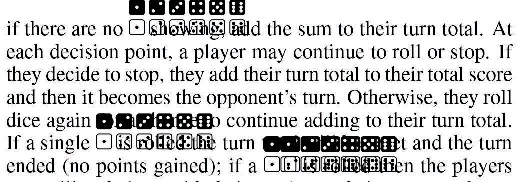
\includegraphics[width=0.9\columnwidth]{figure1} % Reduce the figure size so that it is slightly narrower than the column. Don't use precise values for figure width.This setup will avoid overfull boxes.
\caption{Using the trim and clip commands produces fragile layers that can result in disasters (like this one from an actual paper) when the color space is corrected or the PDF combined with others for the final proceedings. Crop your figures properly in a graphics program -- not in LaTeX.}
\label{fig1}
\end{figure}

\begin{figure*}[t]
\centering
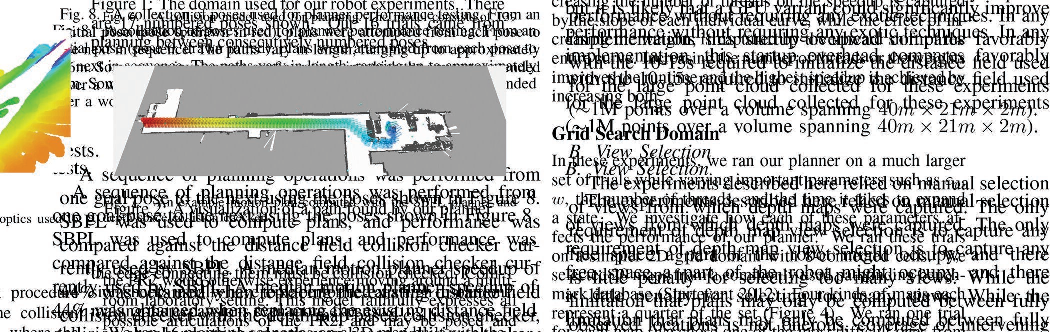
\includegraphics[width=0.8\textwidth]{figure2} % Reduce the figure size so that it is slightly narrower than the column.
\caption{Adjusting the bounding box instead of actually removing the unwanted data resulted multiple layers in this paper. It also needlessly increased the PDF size. In this case, the size of the unwanted layer doubled the paper's size, and produced the following surprising results in final production. Crop your figures properly in a graphics program. Don't just alter the bounding box.}
\label{fig2}
\end{figure*}

% Using the \centering command instead of \begin{center} ... \end{center} will save space
% Positioning your figure at the top of the page will save space and make the paper more readable
% Using 0.95\columnwidth in conjunction with the


Your paper must compile in PDF\LaTeX{}. Consequently, all your figures must be .jpg, .png, or .pdf. You may not use the .gif (the resolution is too low), .ps, or .eps file format for your figures.

Figures, drawings, tables, and photographs should be placed throughout the paper on the page (or the subsequent page) where they are first discussed. Do not group them together at the end of the paper. If placed at the top of the paper, illustrations may run across both columns. Figures must not invade the top, bottom, or side margin areas. Figures must be inserted using the \textbackslash usepackage\{graphicx\}. Number figures sequentially, for example, figure 1, and so on. Do not use minipage to group figures.

If you normally create your figures using pgfplots, please create the figures first, and then import them as pdfs with proper bounding boxes, as the bounding and trim boxes created by pfgplots are fragile and not valid.

When you include your figures, you must crop them \textbf{outside} of \LaTeX{}. The command \textbackslash includegraphics*[clip=true, viewport 0 0 10 10]{...} might result in a PDF that looks great, but the image is \textbf{not really cropped.} The full image can reappear (and obscure whatever it is overlapping) when page numbers are applied or color space is standardized. Figures \ref{fig1}, and \ref{fig2} display some unwanted results that often occur.

If your paper includes illustrations that are not compatible with PDF\TeX{} (such as .eps or .ps documents), you will need to convert them. The epstopdf package will usually work for eps files. You will need to convert your ps files to PDF in either case.

\subsubsection {Figure Captions.}The illustration number and caption must appear \textit{under} the illustration. Labels and other text with the actual illustration must be at least nine-point type. However, the font and size of figure captions must be 10 point roman. Do not make them smaller, bold, or italic. (Individual words may be italicized if the context requires differentiation.)

\subsection{Tables}

Tables should be presented in 10 point roman type. If necessary, they may be altered to 9 point type. You must not use \texttt{\textbackslash resizebox} or other commands that resize the entire table to make it smaller, because you can't control the final font size this way.
If your table is too large you can use \texttt{\textbackslash setlength\{\textbackslash tabcolsep\}\{1mm\}} to compress the columns a bit or you can adapt the content (e.g.: reduce the decimal precision when presenting numbers, use shortened column titles, make some column duble-line to get it narrower).

Tables that do not fit in a single column must be placed across double columns. If your table won't fit within the margins even when spanning both columns and using the above techniques, you must split it in two separate tables.

\subsubsection {Table Captions.} The number and caption for your table must appear \textit{under} (not above) the table.  Additionally, the font and size of table captions must be 10 point roman and must be placed beneath the figure. Do not make them smaller, bold, or italic. (Individual words may be italicized if the context requires differentiation.)



\subsubsection{Low-Resolution Bitmaps.}
You may not use low-resolution (such as 72 dpi) screen-dumps and GIF files---these files contain so few pixels that they are always blurry, and illegible when printed. If they are color, they will become an indecipherable mess when converted to black and white. This is always the case with gif files, which should never be used. The resolution of screen dumps can be increased by reducing the print size of the original file while retaining the same number of pixels. You can also enlarge files by manipulating them in software such as PhotoShop. Your figures should be 300 dpi when incorporated into your document.

\subsubsection{\LaTeX{} Overflow.}
\LaTeX{} users please beware: \LaTeX{} will sometimes put portions of the figure or table or an equation in the margin. If this happens, you need to make the figure or table span both columns. If absolutely necessary, you may reduce the figure, or reformat the equation, or reconfigure the table.{ \bf Check your log file!} You must fix any overflow into the margin (that means no overfull boxes in \LaTeX{}). \textbf{Nothing is permitted to intrude into the margin or gutter.}


\subsubsection{Using Color.}
Use of color is restricted to figures only. It must be WACG 2.0 compliant. (That is, the contrast ratio must be greater than 4.5:1 no matter the font size.) It must be CMYK, NOT RGB. It may never be used for any portion of the text of your paper. The archival version of your paper will be printed in black and white and grayscale. The web version must be readable by persons with disabilities. Consequently, because conversion to grayscale can cause undesirable effects (red changes to black, yellow can disappear, and so forth), we strongly suggest you avoid placing color figures in your document. If you do include color figures, you must (1) use the CMYK (not RGB) colorspace and (2) be mindful of readers who may happen to have trouble distinguishing colors. Your paper must be decipherable without using color for distinction.

\subsubsection{Drawings.}
We suggest you use computer drawing software (such as Adobe Illustrator or, (if unavoidable), the drawing tools in Microsoft Word) to create your illustrations. Do not use Microsoft Publisher. These illustrations will look best if all line widths are uniform (half- to two-point in size), and you do not create labels over shaded areas. Shading should be 133 lines per inch if possible. Use Times Roman or Helvetica for all figure call-outs. \textbf{Do not use hairline width lines} --- be sure that the stroke width of all lines is at least .5 pt. Zero point lines will print on a laser printer, but will completely disappear on the high-resolution devices used by our printers.

\subsubsection{Photographs and Images.}
Photographs and other images should be in grayscale (color photographs will not reproduce well; for example, red tones will reproduce as black, yellow may turn to white, and so forth) and set to a minimum of 300 dpi. Do not prescreen images.

\subsubsection{Resizing Graphics.}
Resize your graphics \textbf{before} you include them with LaTeX. You may \textbf{not} use trim or clip options as part of your \textbackslash includegraphics command. Resize the media box of your PDF using a graphics program instead.

\subsubsection{Fonts in Your Illustrations.}
You must embed all fonts in your graphics before including them in your LaTeX document.

\subsubsection{Algorithms.}
Algorithms and/or programs are a special kind of figures. Like all illustrations, they should appear floated to the top (preferably) or bottom of the page. However, their caption should appear in the header, left-justified and enclosed between horizontal lines, as shown in Algorithm~\ref{alg:algorithm}. The algorithm body should be terminated with another horizontal line. It is up to the authors to decide whether to show line numbers or not, how to format comments, etc.

In \LaTeX{} algorithms may be typeset using the {\tt algorithm} and {\tt algorithmic} packages, but you can also use one of the many other packages for the task.

\begin{algorithm}[tb]
\caption{Example algorithm}
\label{alg:algorithm}
\textbf{Input}: Your algorithm's input\\
\textbf{Parameter}: Optional list of parameters\\
\textbf{Output}: Your algorithm's output
\begin{algorithmic}[1] %[1] enables line numbers
\STATE Let $t=0$.
\WHILE{condition}
\STATE Do some action.
\IF {conditional}
\STATE Perform task A.
\ELSE
\STATE Perform task B.
\ENDIF
\ENDWHILE
\STATE \textbf{return} solution
\end{algorithmic}
\end{algorithm}

\subsubsection{Listings.}
Listings are much like algorithms and programs. They should also appear floated to the top (preferably) or bottom of the page. Listing captions should appear in the header, left-justified and enclosed between horizontal lines as shown in Listing~\ref{lst:listing}. Terminate the body with another horizontal line and avoid any background color. Line numbers, if included, must appear within the text column.

\begin{listing}[tb]%
\caption{Example listing {\tt quicksort.hs}}%
\label{lst:listing}%
\begin{lstlisting}[language=Haskell]
quicksort :: Ord a => [a] -> [a]
quicksort []     = []
quicksort (p:xs) = (quicksort lesser) ++ [p] ++ (quicksort greater)
	where
		lesser  = filter (< p) xs
		greater = filter (>= p) xs
\end{lstlisting}
\end{listing}

\subsection{References}
The AAAI style includes a set of definitions for use in formatting references with BibTeX. These definitions make the bibliography style fairly close to the ones  specified in the Reference Examples appendix below. To use these definitions, you also need the BibTeX style file ``aaai2026.bst," available in the AAAI Author Kit on the AAAI web site. Then, at the end of your paper but before \textbackslash end{document}, you need to put the following lines:

\begin{quote}
\begin{small}
\textbackslash bibliography\{bibfile1,bibfile2,...\}
\end{small}
\end{quote}

Please note that the aaai2026.sty class already sets the bibliographystyle for you, so you do not have to place any \textbackslash bibliographystyle command in the document yourselves. The aaai2026.sty file is incompatible with the hyperref and navigator packages. If you use either, your references will be garbled and your paper will be returned to you.

References may be the same size as surrounding text.
However, in this section (only), you may reduce the size to {\em \textbackslash small} (9pt) if your paper exceeds the allowable number of pages. Making it any smaller than 9 point with 10 point linespacing, however, is not allowed.

The list of files in the \textbackslash bibliography command should be the names of your BibTeX source files (that is, the .bib files referenced in your paper).

The following commands are available for your use in citing references:
\begin{quote}
{\em \textbackslash cite:} Cites the given reference(s) with a full citation. This appears as ``(Author Year)'' for one reference, or ``(Author Year; Author Year)'' for multiple references.\smallskip\\
{\em \textbackslash shortcite:} Cites the given reference(s) with just the year. This appears as ``(Year)'' for one reference, or ``(Year; Year)'' for multiple references.\smallskip\\
{\em \textbackslash citeauthor:} Cites the given reference(s) with just the author name(s) and no parentheses.\smallskip\\
{\em \textbackslash citeyear:} Cites the given reference(s) with just the date(s) and no parentheses.
\end{quote}
You may also use any of the \emph{natbib} citation commands.


\section{Proofreading Your PDF}
Please check all the pages of your PDF file. The most commonly forgotten element is the acknowledgements --- especially the correct grant number. Authors also commonly forget to add the metadata to the source, use the wrong reference style file, or don't follow the capitalization rules or comma placement for their author-title information properly. A final common problem is text (expecially equations) that runs into the margin. You will need to fix these common errors before submitting your file.

\section{Improperly Formatted Files }
In the past, AAAI has corrected improperly formatted files submitted by the authors. Unfortunately, this has become an increasingly burdensome expense that we can no longer absorb). Consequently, if your file is improperly formatted, it will be returned to you for correction.

\section{Naming Your Electronic File}
We require that you name your \LaTeX{} source file with the last name (family name) of the first author so that it can easily be differentiated from other submissions. Complete file-naming instructions will be provided to you in the submission instructions.

\section{Submitting Your Electronic Files to AAAI}
Instructions on paper submittal will be provided to you in your acceptance letter.

\section{Inquiries}
If you have any questions about the preparation or submission of your paper as instructed in this document, please contact AAAI Press at the address given below. If you have technical questions about implementation of the aaai style file, please contact an expert at your site. We do not provide technical support for \LaTeX{} or any other software package. To avoid problems, please keep your paper simple, and do not incorporate complicated macros and style files.

\begin{quote}
\noindent AAAI Press\\
1101 Pennsylvania Ave, NW Suite 300\\
Washington, DC 20004 USA\\
\textit{Telephone:} 1-202-360-4062\\
\textit{E-mail:} See the submission instructions for your particular conference or event.
\end{quote}

\section{Additional Resources}
\LaTeX{} is a difficult program to master. If you've used that software, and this document didn't help or some items were not explained clearly, we recommend you read Michael Shell's excellent document (testflow doc.txt V1.0a 2002/08/13) about obtaining correct PS/PDF output on \LaTeX{} systems. (It was written for another purpose, but it has general application as well). It is available at www.ctan.org in the tex-archive.

\appendix
\section{Reference Examples}
\label{sec:reference_examples}

\nobibliography*
Formatted bibliographies should look like the following examples. You should use BibTeX to generate the references. Missing fields are unacceptable when compiling references, and usually indicate that you are using the wrong type of entry (BibTeX class).

\paragraph{Book with multiple authors~\nocite{em:86}} Use the \texttt{@book} class.\\[.2em]
\bibentry{em:86}.

\paragraph{Journal and magazine articles~\nocite{r:80, hcr:83}} Use the \texttt{@article} class.\\[.2em]
\bibentry{r:80}.\\[.2em]
\bibentry{hcr:83}.

\paragraph{Proceedings paper published by a society, press or publisher~\nocite{c:83, c:84}} Use the \texttt{@inproceedings} class. You may abbreviate the \emph{booktitle} field, but make sure that the conference edition is clear.\\[.2em]
\bibentry{c:84}.\\[.2em]
\bibentry{c:83}.

\paragraph{University technical report~\nocite{r:86}} Use the \texttt{@techreport} class.\\[.2em]
\bibentry{r:86}.

\paragraph{Dissertation or thesis~\nocite{c:79}} Use the \texttt{@phdthesis} class.\\[.2em]
\bibentry{c:79}.

\paragraph{Forthcoming publication~\nocite{c:21}} Use the \texttt{@misc} class with a \texttt{note="Forthcoming"} annotation.
\begin{quote}
\begin{footnotesize}
\begin{verbatim}
@misc(key,
  [...]
  note="Forthcoming",
)
\end{verbatim}
\end{footnotesize}
\end{quote}
\bibentry{c:21}.

\paragraph{ArXiv paper~\nocite{c:22}} Fetch the BibTeX entry from the "Export Bibtex Citation" link in the arXiv website. Notice it uses the \texttt{@misc} class instead of the \texttt{@article} one, and that it includes the \texttt{eprint} and \texttt{archivePrefix} keys.
\begin{quote}
\begin{footnotesize}
\begin{verbatim}
@misc(key,
  [...]
  eprint="xxxx.yyyy",
  archivePrefix="arXiv",
)
\end{verbatim}
\end{footnotesize}
\end{quote}
\bibentry{c:22}.

\paragraph{Website or online resource~\nocite{c:23}} Use the \texttt{@misc} class. Add the url in the \texttt{howpublished} field and the date of access in the \texttt{note} field:
\begin{quote}
\begin{footnotesize}
\begin{verbatim}
@misc(key,
  [...]
  howpublished="\url{http://...}",
  note="Accessed: YYYY-mm-dd",
)
\end{verbatim}
\end{footnotesize}
\end{quote}
\bibentry{c:23}.

For the most up to date version of the AAAI reference style, please consult the \textit{AI Magazine} Author Guidelines at \url{https://aaai.org/ojs/index.php/aimagazine/about/submissions#authorGuidelines}

\section{Acknowledgments}
AAAI is especially grateful to Peter Patel Schneider for his work in implementing the original aaai.sty file, liberally using the ideas of other style hackers, including Barbara Beeton. We also acknowledge with thanks the work of George Ferguson for his guide to using the style and BibTeX files --- which has been incorporated into this document --- and Hans Guesgen, who provided several timely modifications, as well as the many others who have, from time to time, sent in suggestions on improvements to the AAAI style. We are especially grateful to Francisco Cruz, Marc Pujol-Gonzalez, and Mico Loretan for the improvements to the Bib\TeX{} and \LaTeX{} files made in 2020.

The preparation of the \LaTeX{} and Bib\TeX{} files that implement these instructions was supported by Schlumberger Palo Alto Research, AT\&T Bell Laboratories, Morgan Kaufmann Publishers, The Live Oak Press, LLC, and AAAI Press. Bibliography style changes were added by Sunil Issar. \verb+\+pubnote was added by J. Scott Penberthy. George Ferguson added support for printing the AAAI copyright slug. Additional changes to aaai2026.sty and aaai2026.bst have been made by Francisco Cruz, Marc Pujol-Gonzalez, and Mico Loretan.

\bigskip
\noindent Thank you for reading these instructions carefully. We look forward to receiving your electronic files!

\bibliography{aaai2026}

\end{document}
